% BSC and BEC diagrams, and their capacities.
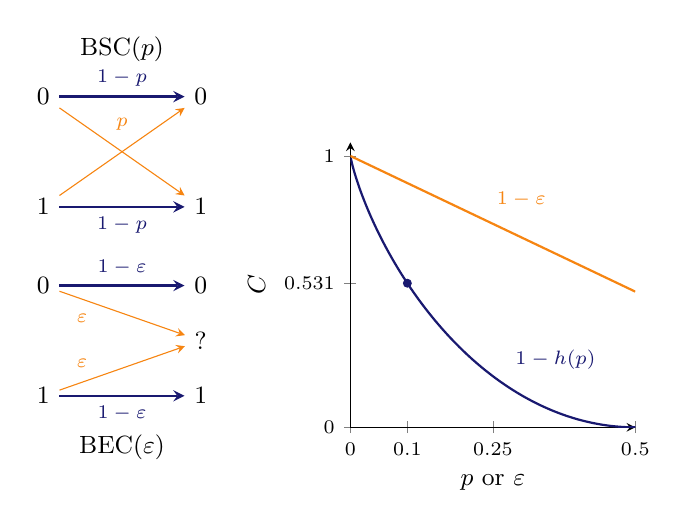
\begin{tikzpicture}[>=stealth,font=\small]
\begin{scope}
\node (a0) at (0,2.6) {$0$}; \node (a1) at (0,1.2) {$1$};
\node (b0) at (2,2.6) {$0$}; \node (b1) at (2,1.2) {$1$};
\draw[->,MidnightBlue,thick] (a0)--node[above]{\scriptsize$1-p$}(b0);
\draw[->,MidnightBlue,thick] (a1)--node[below]{\scriptsize$1-p$}(b1);
\draw[->,BurntOrange] (a0)--(b1); \draw[->,BurntOrange] (a1)--(b0);
\node[BurntOrange] at (1,2.25) {\scriptsize$p$};
\node at (1,3.2) {$\mathrm{BSC}(p)$};
\node (c0) at (0,0.2) {$0$}; \node (c1) at (0,-1.2) {$1$};
\node (d0) at (2,0.2) {$0$}; \node (de) at (2,-0.5) {$?$}; \node (d1) at (2,-1.2) {$1$};
\draw[->,MidnightBlue,thick] (c0)--node[above]{\scriptsize$1-\varepsilon$}(d0);
\draw[->,MidnightBlue,thick] (c1)--node[below]{\scriptsize$1-\varepsilon$}(d1);
\draw[->,BurntOrange] (c0)--node[pos=0.3,below left]{\scriptsize$\varepsilon$}(de);
\draw[->,BurntOrange] (c1)--node[pos=0.3,above left]{\scriptsize$\varepsilon$}(de);
\node at (1,-1.85) {$\mathrm{BEC}(\varepsilon)$};
\end{scope}
\begin{scope}[xshift=3.9cm,yshift=-1.6cm]
\begin{axis}[width=5.2cm,height=5.2cm,xmin=0,xmax=0.5,ymin=0,ymax=1.05,
  xlabel={$p$ or $\varepsilon$},ylabel={$C$},xtick={0,0.1,0.25,0.5},ytick={0,0.531,1},
  yticklabels={$0$,$0.531$,$1$},axis lines=left,tick label style={font=\scriptsize},label style={font=\small}]
\addplot[MidnightBlue,thick,domain=0.0005:0.5,samples=150] {1+x*ln(x)/ln(2)+(1-x)*ln(1-x)/ln(2)};
\node[MidnightBlue,font=\scriptsize] at (axis cs:0.36,0.25) {$1-h(p)$};
\addplot[BurntOrange,thick,domain=0:0.5] {1-x};
\node[BurntOrange,font=\scriptsize] at (axis cs:0.3,0.84) {$1-\varepsilon$};
\addplot[only marks,mark=*,mark size=1.4pt,MidnightBlue] coordinates {(0.1,0.531)};
\end{axis}
\end{scope}
\end{tikzpicture}
